% Created by tikzDevice version 0.12.6 on 2024-06-12 16:03:20
% !TEX encoding = UTF-8 Unicode
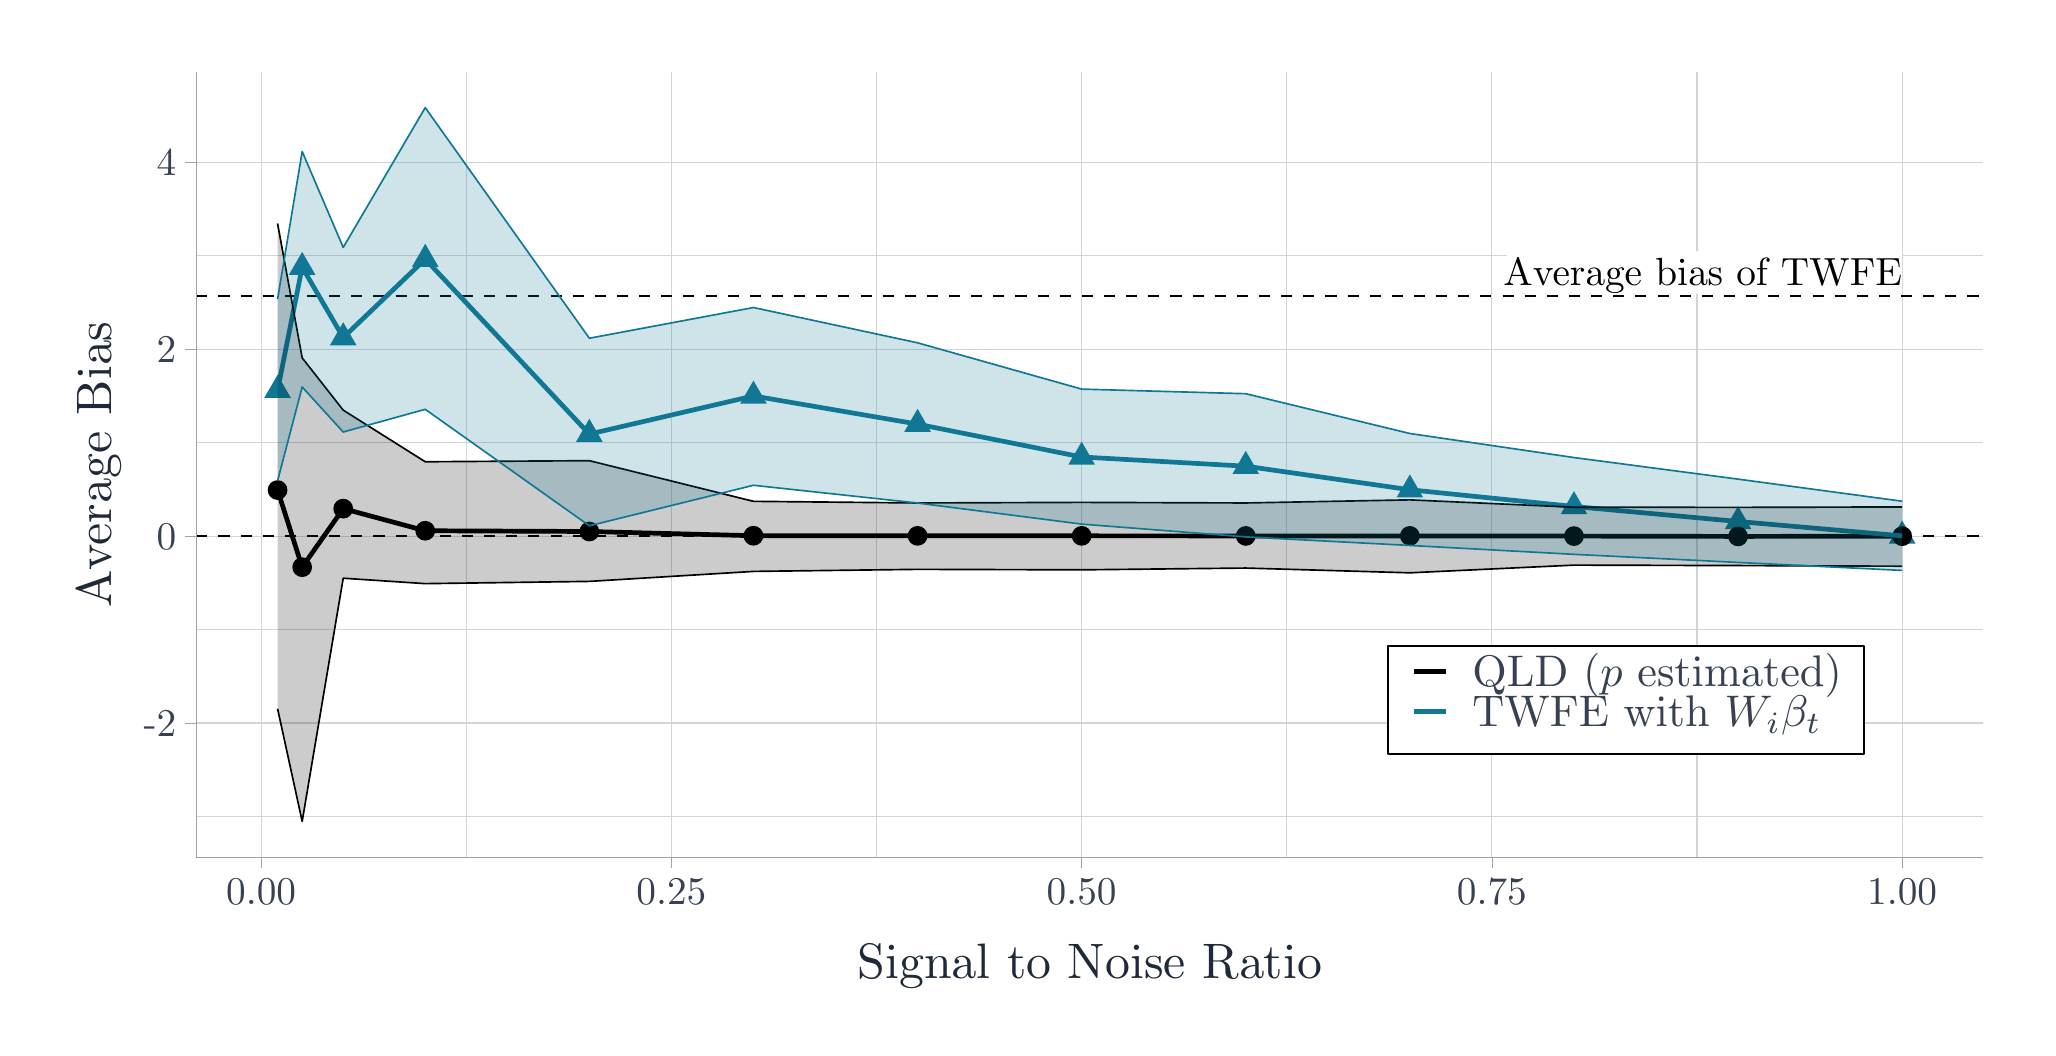
\begin{tikzpicture}[x=1pt,y=1pt]
\definecolor{fillColor}{RGB}{255,255,255}
\path[use as bounding box,fill=fillColor] (0,0) rectangle (722.70,361.35);
\begin{scope}
\path[clip] (  0.00,  0.00) rectangle (722.70,361.35);
\definecolor{drawColor}{RGB}{255,255,255}

\path[draw=drawColor,line width= 0.8pt,line join=round,line cap=round,fill=fillColor] (  0.00,  0.00) rectangle (722.70,361.35);
\end{scope}
\begin{scope}
\path[clip] ( 60.94, 61.65) rectangle (706.70,345.35);
\definecolor{drawColor}{RGB}{255,255,255}
\definecolor{fillColor}{RGB}{255,255,255}

\path[draw=drawColor,line width= 0.8pt,line join=round,line cap=round,fill=fillColor] ( 60.94, 61.65) rectangle (706.70,345.35);
\definecolor{drawColor}{RGB}{209,213,219}

\path[draw=drawColor,line width= 0.4pt,line join=round] ( 60.94, 76.31) --
	(706.70, 76.31);

\path[draw=drawColor,line width= 0.4pt,line join=round] ( 60.94,143.86) --
	(706.70,143.86);

\path[draw=drawColor,line width= 0.4pt,line join=round] ( 60.94,211.41) --
	(706.70,211.41);

\path[draw=drawColor,line width= 0.4pt,line join=round] ( 60.94,278.95) --
	(706.70,278.95);

\path[draw=drawColor,line width= 0.4pt,line join=round] (158.49, 61.65) --
	(158.49,345.35);

\path[draw=drawColor,line width= 0.4pt,line join=round] (306.73, 61.65) --
	(306.73,345.35);

\path[draw=drawColor,line width= 0.4pt,line join=round] (454.98, 61.65) --
	(454.98,345.35);

\path[draw=drawColor,line width= 0.4pt,line join=round] (603.22, 61.65) --
	(603.22,345.35);

\path[draw=drawColor,line width= 0.4pt,line join=round] ( 60.94,110.09) --
	(706.70,110.09);

\path[draw=drawColor,line width= 0.4pt,line join=round] ( 60.94,177.63) --
	(706.70,177.63);

\path[draw=drawColor,line width= 0.4pt,line join=round] ( 60.94,245.18) --
	(706.70,245.18);

\path[draw=drawColor,line width= 0.4pt,line join=round] ( 60.94,312.73) --
	(706.70,312.73);

\path[draw=drawColor,line width= 0.4pt,line join=round] ( 84.37, 61.65) --
	( 84.37,345.35);

\path[draw=drawColor,line width= 0.4pt,line join=round] (232.61, 61.65) --
	(232.61,345.35);

\path[draw=drawColor,line width= 0.4pt,line join=round] (380.86, 61.65) --
	(380.86,345.35);

\path[draw=drawColor,line width= 0.4pt,line join=round] (529.10, 61.65) --
	(529.10,345.35);

\path[draw=drawColor,line width= 0.4pt,line join=round] (677.35, 61.65) --
	(677.35,345.35);
\definecolor{drawColor}{RGB}{0,0,0}

\path[draw=drawColor,line width= 0.6pt,dash pattern=on 4pt off 4pt ,line join=round] ( 60.94,177.63) -- (706.70,177.63);

\path[draw=drawColor,line width= 0.6pt,dash pattern=on 4pt off 4pt ,line join=round] ( 60.94,264.47) -- (706.70,264.47);
\definecolor{fillColor}{RGB}{16,120,149}

\path[fill=fillColor] ( 90.30,235.90) --
	( 95.10,227.58) --
	( 85.49,227.58) --
	cycle;
\definecolor{fillColor}{RGB}{0,0,0}

\path[fill=fillColor] ( 90.30,194.27) circle (  3.57);
\definecolor{fillColor}{RGB}{16,120,149}

\path[fill=fillColor] ( 99.19,280.34) --
	(104.00,272.01) --
	( 94.38,272.01) --
	cycle;
\definecolor{fillColor}{RGB}{0,0,0}

\path[fill=fillColor] ( 99.19,166.40) circle (  3.57);
\definecolor{fillColor}{RGB}{16,120,149}

\path[fill=fillColor] (114.02,254.91) --
	(118.82,246.58) --
	(109.21,246.58) --
	cycle;
\definecolor{fillColor}{RGB}{0,0,0}

\path[fill=fillColor] (114.02,187.55) circle (  3.57);
\definecolor{fillColor}{RGB}{16,120,149}

\path[fill=fillColor] (143.66,283.26) --
	(148.47,274.93) --
	(138.86,274.93) --
	cycle;
\definecolor{fillColor}{RGB}{0,0,0}

\path[fill=fillColor] (143.66,179.56) circle (  3.57);
\definecolor{fillColor}{RGB}{16,120,149}

\path[fill=fillColor] (202.96,220.03) --
	(207.77,211.70) --
	(198.16,211.70) --
	cycle;
\definecolor{fillColor}{RGB}{0,0,0}

\path[fill=fillColor] (202.96,179.29) circle (  3.57);
\definecolor{fillColor}{RGB}{16,120,149}

\path[fill=fillColor] (262.26,233.82) --
	(267.07,225.50) --
	(257.45,225.50) --
	cycle;
\definecolor{fillColor}{RGB}{0,0,0}

\path[fill=fillColor] (262.26,177.76) circle (  3.57);
\definecolor{fillColor}{RGB}{16,120,149}

\path[fill=fillColor] (321.56,223.64) --
	(326.36,215.32) --
	(316.75,215.32) --
	cycle;
\definecolor{fillColor}{RGB}{0,0,0}

\path[fill=fillColor] (321.56,177.72) circle (  3.57);
\definecolor{fillColor}{RGB}{16,120,149}

\path[fill=fillColor] (380.86,211.76) --
	(385.66,203.44) --
	(376.05,203.44) --
	cycle;
\definecolor{fillColor}{RGB}{0,0,0}

\path[fill=fillColor] (380.86,177.72) circle (  3.57);
\definecolor{fillColor}{RGB}{16,120,149}

\path[fill=fillColor] (440.15,208.44) --
	(444.96,200.11) --
	(435.35,200.11) --
	cycle;
\definecolor{fillColor}{RGB}{0,0,0}

\path[fill=fillColor] (440.15,177.69) circle (  3.57);
\definecolor{fillColor}{RGB}{16,120,149}

\path[fill=fillColor] (499.45,199.92) --
	(504.26,191.59) --
	(494.65,191.59) --
	cycle;
\definecolor{fillColor}{RGB}{0,0,0}

\path[fill=fillColor] (499.45,177.70) circle (  3.57);
\definecolor{fillColor}{RGB}{16,120,149}

\path[fill=fillColor] (558.75,193.88) --
	(563.56,185.56) --
	(553.95,185.56) --
	cycle;
\definecolor{fillColor}{RGB}{0,0,0}

\path[fill=fillColor] (558.75,177.63) circle (  3.57);
\definecolor{fillColor}{RGB}{16,120,149}

\path[fill=fillColor] (618.05,188.46) --
	(622.86,180.13) --
	(613.24,180.13) --
	cycle;
\definecolor{fillColor}{RGB}{0,0,0}

\path[fill=fillColor] (618.05,177.51) circle (  3.57);
\definecolor{fillColor}{RGB}{16,120,149}

\path[fill=fillColor] (677.35,183.27) --
	(682.15,174.95) --
	(672.54,174.95) --
	cycle;
\definecolor{fillColor}{RGB}{0,0,0}

\path[fill=fillColor] (677.35,177.61) circle (  3.57);

\path[draw=drawColor,line width= 1.7pt,line join=round] ( 90.30,194.27) --
	( 99.19,166.40) --
	(114.02,187.55) --
	(143.66,179.56) --
	(202.96,179.29) --
	(262.26,177.76) --
	(321.56,177.72) --
	(380.86,177.72) --
	(440.15,177.69) --
	(499.45,177.70) --
	(558.75,177.63) --
	(618.05,177.51) --
	(677.35,177.61);
\definecolor{drawColor}{RGB}{16,120,149}

\path[draw=drawColor,line width= 1.7pt,line join=round] ( 90.30,230.35) --
	( 99.19,274.79) --
	(114.02,249.36) --
	(143.66,277.71) --
	(202.96,214.48) --
	(262.26,228.27) --
	(321.56,218.09) --
	(380.86,206.21) --
	(440.15,202.89) --
	(499.45,194.37) --
	(558.75,188.33) --
	(618.05,182.91) --
	(677.35,177.72);
\definecolor{fillColor}{RGB}{0,0,0}

\path[fill=fillColor,fill opacity=0.20] ( 90.30,290.59) --
	( 99.19,242.03) --
	(114.02,223.14) --
	(143.66,204.49) --
	(202.96,204.88) --
	(262.26,190.19) --
	(321.56,189.60) --
	(380.86,189.81) --
	(440.15,189.60) --
	(499.45,190.72) --
	(558.75,188.06) --
	(618.05,188.01) --
	(677.35,188.16) --
	(677.35,166.75) --
	(618.05,166.98) --
	(558.75,167.14) --
	(499.45,164.36) --
	(440.15,166.08) --
	(380.86,165.44) --
	(321.56,165.61) --
	(262.26,164.87) --
	(202.96,161.26) --
	(143.66,160.45) --
	(114.02,162.41) --
	( 99.19, 74.55) --
	( 90.30,115.26) --
	cycle;
\definecolor{drawColor}{RGB}{0,0,0}

\path[draw=drawColor,line width= 0.6pt,line join=round] ( 90.30,290.59) --
	( 99.19,242.03) --
	(114.02,223.14) --
	(143.66,204.49) --
	(202.96,204.88) --
	(262.26,190.19) --
	(321.56,189.60) --
	(380.86,189.81) --
	(440.15,189.60) --
	(499.45,190.72) --
	(558.75,188.06) --
	(618.05,188.01) --
	(677.35,188.16);

\path[draw=drawColor,line width= 0.6pt,line join=round] (677.35,166.75) --
	(618.05,166.98) --
	(558.75,167.14) --
	(499.45,164.36) --
	(440.15,166.08) --
	(380.86,165.44) --
	(321.56,165.61) --
	(262.26,164.87) --
	(202.96,161.26) --
	(143.66,160.45) --
	(114.02,162.41) --
	( 99.19, 74.55) --
	( 90.30,115.26);
\definecolor{fillColor}{RGB}{16,120,149}

\path[fill=fillColor,fill opacity=0.20] ( 90.30,263.24) --
	( 99.19,316.60) --
	(114.02,281.93) --
	(143.66,332.45) --
	(202.96,249.12) --
	(262.26,260.22) --
	(321.56,247.47) --
	(380.86,230.74) --
	(440.15,229.08) --
	(499.45,214.70) --
	(558.75,206.01) --
	(618.05,198.21) --
	(677.35,190.23) --
	(677.35,165.23) --
	(618.05,168.11) --
	(558.75,171.04) --
	(499.45,174.25) --
	(440.15,177.34) --
	(380.86,181.96) --
	(321.56,189.58) --
	(262.26,195.99) --
	(202.96,181.36) --
	(143.66,223.44) --
	(114.02,215.24) --
	( 99.19,231.51) --
	( 90.30,197.58) --
	cycle;
\definecolor{drawColor}{RGB}{16,120,149}

\path[draw=drawColor,line width= 0.6pt,line join=round] ( 90.30,263.24) --
	( 99.19,316.60) --
	(114.02,281.93) --
	(143.66,332.45) --
	(202.96,249.12) --
	(262.26,260.22) --
	(321.56,247.47) --
	(380.86,230.74) --
	(440.15,229.08) --
	(499.45,214.70) --
	(558.75,206.01) --
	(618.05,198.21) --
	(677.35,190.23);

\path[draw=drawColor,line width= 0.6pt,line join=round] (677.35,165.23) --
	(618.05,168.11) --
	(558.75,171.04) --
	(499.45,174.25) --
	(440.15,177.34) --
	(380.86,181.96) --
	(321.56,189.58) --
	(262.26,195.99) --
	(202.96,181.36) --
	(143.66,223.44) --
	(114.02,215.24) --
	( 99.19,231.51) --
	( 90.30,197.58);
\definecolor{fillColor}{RGB}{255,255,255}

\path[fill=fillColor] (534.57,265.25) --
	(677.35,265.25) --
	(677.35,265.25) --
	(677.35,265.25) --
	(677.35,265.25) --
	(677.35,265.25) --
	(677.35,265.25) --
	(677.35,265.25) --
	(677.35,265.25) --
	(677.35,265.25) --
	(677.35,265.25) --
	(677.35,265.25) --
	(677.35,265.25) --
	(677.35,265.25) --
	(677.35,280.58) --
	(677.35,280.58) --
	(677.35,280.58) --
	(677.35,280.58) --
	(677.35,280.58) --
	(677.35,280.58) --
	(677.35,280.58) --
	(677.35,280.58) --
	(677.35,280.58) --
	(677.35,280.58) --
	(677.35,280.58) --
	(677.35,280.58) --
	(534.57,280.58) --
	(534.57,280.58) --
	(534.57,280.58) --
	(534.57,280.58) --
	(534.57,280.58) --
	(534.57,280.58) --
	(534.57,280.58) --
	(534.57,280.58) --
	(534.57,280.58) --
	(534.57,280.58) --
	(534.57,280.58) --
	(534.57,280.58) --
	(534.57,280.58) --
	(534.57,265.25) --
	(534.57,265.25) --
	(534.57,265.25) --
	(534.57,265.25) --
	(534.57,265.25) --
	(534.57,265.25) --
	(534.57,265.25) --
	(534.57,265.25) --
	(534.57,265.25) --
	(534.57,265.25) --
	(534.57,265.25) --
	(534.57,265.25) --
	cycle;
\end{scope}
\begin{scope}
\path[clip] ( 60.94, 61.65) rectangle (706.70,345.35);
\definecolor{drawColor}{RGB}{0,0,0}

\node[text=drawColor,anchor=base east,inner sep=0pt, outer sep=0pt, scale=  1.42] at (677.35,268.01) {Average bias of TWFE};
\end{scope}
\begin{scope}
\path[clip] (  0.00,  0.00) rectangle (722.70,361.35);
\definecolor{drawColor}{RGB}{156,163,175}

\path[draw=drawColor,line width= 0.3pt,line join=round] ( 60.94, 61.65) --
	( 60.94,345.35);
\end{scope}
\begin{scope}
\path[clip] (  0.00,  0.00) rectangle (722.70,361.35);
\definecolor{drawColor}{RGB}{55,65,81}

\node[text=drawColor,anchor=base east,inner sep=0pt, outer sep=0pt, scale=  1.42] at ( 53.74,105.19) {-2};

\node[text=drawColor,anchor=base east,inner sep=0pt, outer sep=0pt, scale=  1.42] at ( 53.74,172.74) {0};

\node[text=drawColor,anchor=base east,inner sep=0pt, outer sep=0pt, scale=  1.42] at ( 53.74,240.28) {2};

\node[text=drawColor,anchor=base east,inner sep=0pt, outer sep=0pt, scale=  1.42] at ( 53.74,307.83) {4};
\end{scope}
\begin{scope}
\path[clip] (  0.00,  0.00) rectangle (722.70,361.35);
\definecolor{drawColor}{RGB}{156,163,175}

\path[draw=drawColor,line width= 0.3pt,line join=round] ( 56.94,110.09) --
	( 60.94,110.09);

\path[draw=drawColor,line width= 0.3pt,line join=round] ( 56.94,177.63) --
	( 60.94,177.63);

\path[draw=drawColor,line width= 0.3pt,line join=round] ( 56.94,245.18) --
	( 60.94,245.18);

\path[draw=drawColor,line width= 0.3pt,line join=round] ( 56.94,312.73) --
	( 60.94,312.73);
\end{scope}
\begin{scope}
\path[clip] (  0.00,  0.00) rectangle (722.70,361.35);
\definecolor{drawColor}{RGB}{156,163,175}

\path[draw=drawColor,line width= 0.3pt,line join=round] ( 60.94, 61.65) --
	(706.70, 61.65);
\end{scope}
\begin{scope}
\path[clip] (  0.00,  0.00) rectangle (722.70,361.35);
\definecolor{drawColor}{RGB}{156,163,175}

\path[draw=drawColor,line width= 0.3pt,line join=round] ( 84.37, 57.65) --
	( 84.37, 61.65);

\path[draw=drawColor,line width= 0.3pt,line join=round] (232.61, 57.65) --
	(232.61, 61.65);

\path[draw=drawColor,line width= 0.3pt,line join=round] (380.86, 57.65) --
	(380.86, 61.65);

\path[draw=drawColor,line width= 0.3pt,line join=round] (529.10, 57.65) --
	(529.10, 61.65);

\path[draw=drawColor,line width= 0.3pt,line join=round] (677.35, 57.65) --
	(677.35, 61.65);
\end{scope}
\begin{scope}
\path[clip] (  0.00,  0.00) rectangle (722.70,361.35);
\definecolor{drawColor}{RGB}{55,65,81}

\node[text=drawColor,anchor=base,inner sep=0pt, outer sep=0pt, scale=  1.42] at ( 84.37, 44.66) {0.00};

\node[text=drawColor,anchor=base,inner sep=0pt, outer sep=0pt, scale=  1.42] at (232.61, 44.66) {0.25};

\node[text=drawColor,anchor=base,inner sep=0pt, outer sep=0pt, scale=  1.42] at (380.86, 44.66) {0.50};

\node[text=drawColor,anchor=base,inner sep=0pt, outer sep=0pt, scale=  1.42] at (529.10, 44.66) {0.75};

\node[text=drawColor,anchor=base,inner sep=0pt, outer sep=0pt, scale=  1.42] at (677.35, 44.66) {1.00};
\end{scope}
\begin{scope}
\path[clip] (  0.00,  0.00) rectangle (722.70,361.35);
\definecolor{drawColor}{RGB}{31,41,55}

\node[text=drawColor,anchor=base,inner sep=0pt, outer sep=0pt, scale=  1.80] at (383.82, 17.75) {Signal to Noise Ratio};
\end{scope}
\begin{scope}
\path[clip] (  0.00,  0.00) rectangle (722.70,361.35);
\definecolor{drawColor}{RGB}{31,41,55}

\node[text=drawColor,rotate= 90.00,anchor=base,inner sep=0pt, outer sep=0pt, scale=  1.80] at ( 30.15,203.50) {Average Bias};
\end{scope}
\begin{scope}
\path[clip] (  0.00,  0.00) rectangle (722.70,361.35);
\definecolor{drawColor}{RGB}{0,0,0}
\definecolor{fillColor}{RGB}{255,255,255}

\path[draw=drawColor,line width= 0.6pt,line join=round,line cap=round,fill=fillColor] (491.60, 98.94) rectangle (663.50,137.85);
\end{scope}
\begin{scope}
\path[clip] (  0.00,  0.00) rectangle (722.70,361.35);
\definecolor{drawColor}{RGB}{255,255,255}
\definecolor{fillColor}{RGB}{255,255,255}

\path[draw=drawColor,line width= 0.8pt,line join=round,line cap=round,fill=fillColor] (499.60,121.39) rectangle (514.05,135.85);
\end{scope}
\begin{scope}
\path[clip] (  0.00,  0.00) rectangle (722.70,361.35);
\definecolor{fillColor}{RGB}{0,0,0}

\path[fill=fillColor] (506.83,128.62) circle (  0.36);
\end{scope}
\begin{scope}
\path[clip] (  0.00,  0.00) rectangle (722.70,361.35);
\definecolor{drawColor}{RGB}{0,0,0}

\path[draw=drawColor,line width= 1.7pt,line join=round] (501.05,128.62) -- (512.61,128.62);
\end{scope}
\begin{scope}
\path[clip] (  0.00,  0.00) rectangle (722.70,361.35);
\definecolor{drawColor}{RGB}{255,255,255}
\definecolor{fillColor}{RGB}{255,255,255}

\path[draw=drawColor,line width= 0.8pt,line join=round,line cap=round,fill=fillColor] (499.60,106.94) rectangle (514.05,121.39);
\end{scope}
\begin{scope}
\path[clip] (  0.00,  0.00) rectangle (722.70,361.35);
\definecolor{fillColor}{RGB}{16,120,149}

\path[fill=fillColor] (506.83,114.72) --
	(507.31,113.89) --
	(506.35,113.89) --
	cycle;
\end{scope}
\begin{scope}
\path[clip] (  0.00,  0.00) rectangle (722.70,361.35);
\definecolor{drawColor}{RGB}{16,120,149}

\path[draw=drawColor,line width= 1.7pt,line join=round] (501.05,114.17) -- (512.61,114.17);
\end{scope}
\begin{scope}
\path[clip] (  0.00,  0.00) rectangle (722.70,361.35);
\definecolor{drawColor}{RGB}{55,65,81}

\node[text=drawColor,anchor=base west,inner sep=0pt, outer sep=0pt, scale=  1.60] at (522.05,123.11) {QLD ($p$ estimated)};
\end{scope}
\begin{scope}
\path[clip] (  0.00,  0.00) rectangle (722.70,361.35);
\definecolor{drawColor}{RGB}{55,65,81}

\node[text=drawColor,anchor=base west,inner sep=0pt, outer sep=0pt, scale=  1.60] at (522.05,108.66) {TWFE with $\bm{W}_i \beta_t$};
\end{scope}
\end{tikzpicture}
